\subsection{Power Functions}
\begin{definition}[Power Functions]
  Any function of the form $f(x) = ax^n$, where $x$ is a variable base, $a$ is a constant coefficient, and $n$ is a real number exponent.
\end{definition}

\textbf{Note: } If $n$ is odd the keypoints are:
\begin{itemize}
\item $(-1, -1)$
\item $(0, 0)$
\item $(1, 1)$
\end{itemize}
If $n$ is even the keypoints are:
\begin{itemize}
\item $(-1, 1)$
\item $(0, 0)$
\item $(1, 1)$
\end{itemize}

\begin{example}[Power Functions]
  \hfill
  \begin{enumerate}
  \item $f(x) = x$
    \begin{center}
      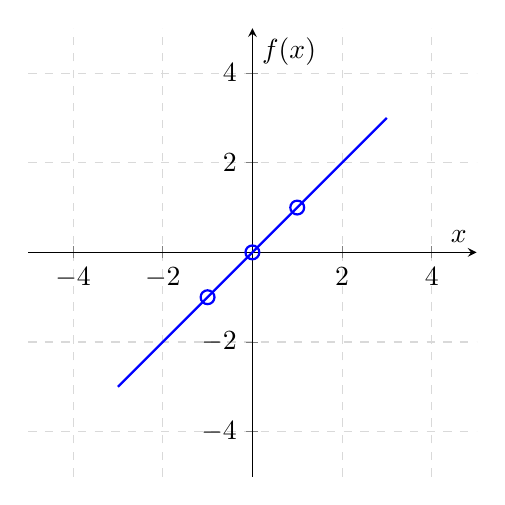
\begin{tikzpicture}
        \begin{axis}[
	    axis lines = center,
	    xlabel = $x$,
	    ylabel = $f(x)$,
	    xmin = -5, xmax = 5,
	    ymin = -5, ymax = 5,
	    grid = major,
	    grid style = {dashed, gray!30},
	    axis equal image
	  ]
	  \addplot [domain=-3:3, samples=100, thick, blue] {x};
          \draw[blue, thick] (axis cs:-1, -1) circle(2.5pt);
          \draw[blue, thick] (axis cs:0, 0) circle(2.5pt);
          \draw[blue, thick] (axis cs:1, 1) circle(2.5pt);
        \end{axis}
      \end{tikzpicture}
    \end{center}
  \item $f(x) = x^2$
    \begin{center}
      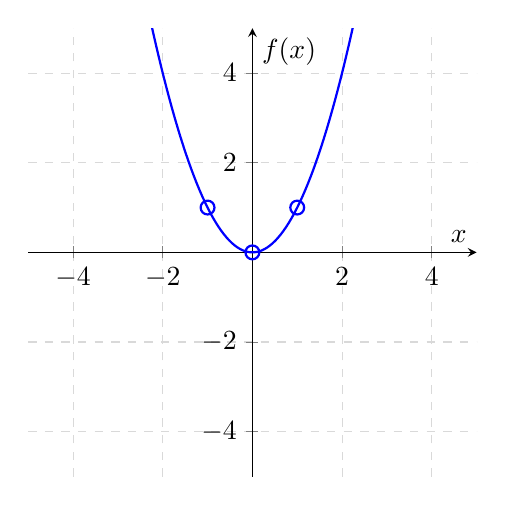
\begin{tikzpicture}
        \begin{axis}[
	    axis lines = center,
	    xlabel = $x$,
	    ylabel = $f(x)$,
	    xmin = -5, xmax = 5,
	    ymin = -5, ymax = 5,
	    grid = major,
	    grid style = {dashed, gray!30},
	    axis equal image
	  ]
	  \addplot [domain=-3:3, samples=100, thick, blue] {x^2};
          \draw[blue, thick] (axis cs:-1, 1) circle(2.5pt);
          \draw[blue, thick] (axis cs:0, 0) circle(2.5pt);
          \draw[blue, thick] (axis cs:1, 1) circle(2.5pt);
        \end{axis}
      \end{tikzpicture}
    \end{center}
  \item $f(x) = x^3$
    \begin{center}
      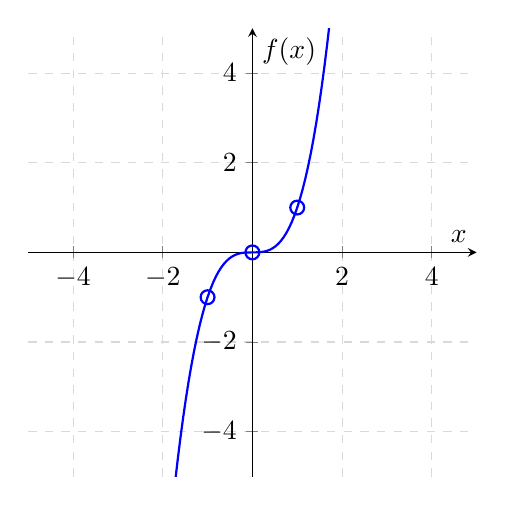
\begin{tikzpicture}
        \begin{axis}[
	    axis lines = center,
	    xlabel = $x$,
	    ylabel = $f(x)$,
	    xmin = -5, xmax = 5,
	    ymin = -5, ymax = 5,
	    grid = major,
	    grid style = {dashed, gray!30},
	    axis equal image
	  ]
	  \addplot [domain=-3:3, samples=100, thick, blue] {x^3};
          \draw[blue, thick] (axis cs:-1, -1) circle(2.5pt);
          \draw[blue, thick] (axis cs:0, 0) circle(2.5pt);
          \draw[blue, thick] (axis cs:1, 1) circle(2.5pt);
        \end{axis}
      \end{tikzpicture}
    \end{center}
  \item $f(x) = x^4$
    \begin{center}
      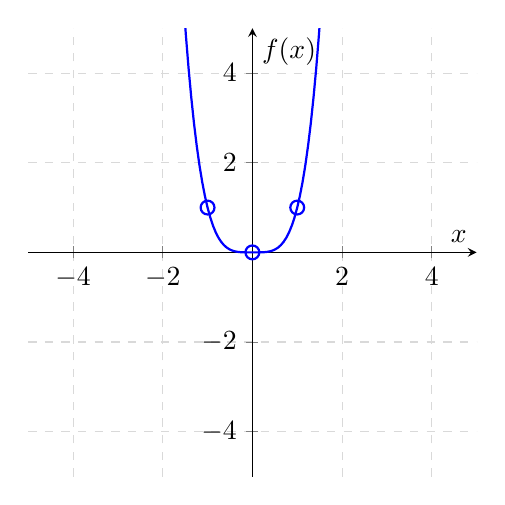
\begin{tikzpicture}
        \begin{axis}[
	    axis lines = center,
	    xlabel = $x$,
	    ylabel = $f(x)$,
	    xmin = -5, xmax = 5,
	    ymin = -5, ymax = 5,
	    grid = major,
	    grid style = {dashed, gray!30},
	    axis equal image
	  ]
	  \addplot [domain=-3:3, samples=100, thick, blue] {x^4};
          \draw[blue, thick] (axis cs:-1, 1) circle(2.5pt);
          \draw[blue, thick] (axis cs:0, 0) circle(2.5pt);
          \draw[blue, thick] (axis cs:1, 1) circle(2.5pt);
        \end{axis}
      \end{tikzpicture}
    \end{center}
  \end{enumerate}
\end{example}

\textbf{Note: }Domain are all $\R$ numbers. so the range for odd functions is:
$$\text{Range: } (-\infty, \infty)$$
While the range for even functions is:
$$\text{Range: } [0, \infty) \lor (-\infty, 0]$$

\begin{example}[Some Other Examples]
  \hfill
  \begin{enumerate}
  \item $G(x) = 3(x  + 2)^5 - 3$ \\
    \begin{center}
      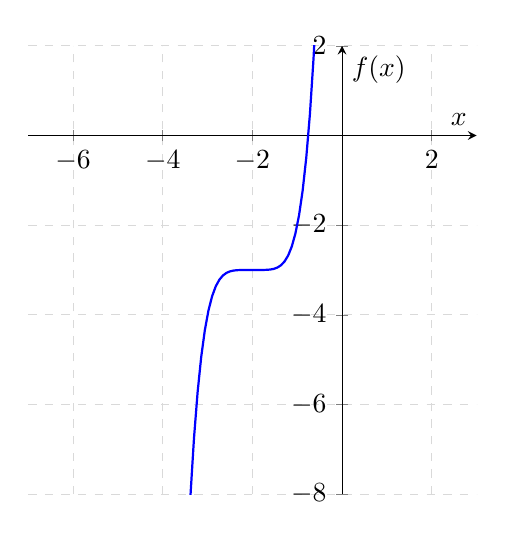
\begin{tikzpicture}
        \begin{axis}[
	    axis lines = center,
	    xlabel = $x$,
	    ylabel = $f(x)$,
	    xmin = -7, xmax = 3,
	    ymin = -8, ymax = 2,
            restrict y to domain = -20:10,
	    grid = major,
	    grid style = {dashed, gray!30},
	    axis equal image
	  ]
	  \addplot [domain=-5:3, samples=100, thick, blue] {3(x+2)^5-3};
        \end{axis}
      \end{tikzpicture}
    \end{center}
  \item  $F(x) = 3 - (x - 2)^4$
    \begin{center}
      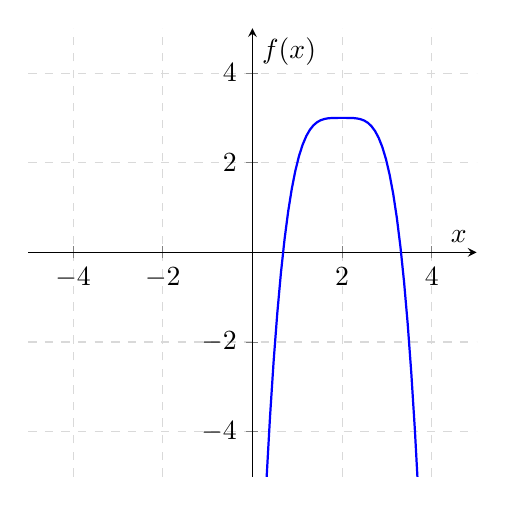
\begin{tikzpicture}
        \begin{axis}[
	    axis lines = center,
	    xlabel = $x$,
	    ylabel = $f(x)$,
	    xmin = -5, xmax = 5,
	    ymin = -5, ymax = 5,
            restrict y to domain = -20:10,
	    grid = major,
	    grid style = {dashed, gray!30},
	    axis equal image
	  ]
	  \addplot [domain=-3:5, samples=100, thick, blue] {3-(x-2)^4};
        \end{axis}
      \end{tikzpicture}
    \end{center}
  \end{enumerate}
\end{example}
